\ProvidesFile{rutitlepage.dtx}[2022/02/21 v3.0 Radboud University Titlepage]
\documentclass{ltxdoc}
\newcommand{\messagespace}{\text{$\mathcal{M}$}}
\newcommand{\messageinstance}{\text{$m$}}
\newcommand{\ciphertextspace}{\text{$\mathcal{C}$}}
\newcommand{\ciphertextinstance}{\text{$c$}}
\newcommand{\associateddataspace}{\text{$\mathcal{A}$}}
\newcommand{\associateddatainstance}{\text{$a$}}
\newcommand{\tagspace}{\text{$\mathcal{T}$}}
\newcommand{\taginstance}{\text{$t$}}
\newcommand{\keyspace}{\text{$\mathcal{K}$}}
\newcommand{\keyinstance}{\text{$k$}}
\newcommand{\noncespace}{\text{$\mathcal{N}$}}
\newcommand{\nonceinstance}{\text{$n$}}
\newcommand{\lockspace}{\text{$\mathcal{L}$}}
\newcommand{\lockinstance}{\text{$l$}}
\newcommand{\users}{\text{$N$}}
\newcommand{\user}{\text{$j$}}
\newcommand{\adversary}{\text{$A$}}
\newcommand{\sample}{\text{$\leftarrow$}}
\newcommand{\result}{\text{$\leftarrow$}}
\newcommand{\concatinate}{\text{$\|$}}

\newcommand{\advantage}[2]{\textbf{Adv}$_{\text{#1}}^{\text{#2}}$ }
\newcommand{\probabilityblock}[4]{\text{$|\text{Pr}[\text{#1}_{\text{#2}}^{\text{#3}}] - \text{Pr}[\text{#1}_{\text{#2}}^{\text{#4}}]|$}}

\newcommand{\pkc}{\text{Hybrid Encryption in a Multi-user Setting, revised}}
\newcommand{\gcrec}{\text{Generic Composition Reconsidered}}

\newcommand{\x}{\text{x}}
\usepackage{a4wide}
\usepackage{float}
\usepackage{graphicx}
\usepackage{array}
\usepackage[utf8]{inputenc}
\usepackage{rutitlepage}
\usepackage{fancyhdr}
\usepackage[style=ieee]{biblatex}
\usepackage[operators]{cryptocode}
\usepackage{amssymb}
\addbibresource{cryptobib/crypto.bib}
\GetFileInfo{rutitlepage.dtx}

\pagestyle{fancy}
\fancyhf{}
\lhead{Bachelor Thesis}
\rhead{Page \thepage}

\title{research proposal}
\author{stijnvandenput }
\date{20 May 2022}

\begin{document}
\maketitleru[
    layout=traditional,
    authors={Stijn Vandenput},
    authorstext={Author:},
    nextpagenr={-1},
    date={20/05/2022},
    institution={Radboud University},
    others={Supervisors:}{Martijn Stam\\Bart Mennink},
    course={Bachelor Thesis},
    title={TBD}]

\section*{Abstract}

\pagenumbering{roman}
\newpage
\tableofcontents

\newpage
\pagenumbering{arabic}

\section{Introduction}
Although symmetric and asymmetric cryptography are both subfields of cryptography, their research area's can be quite separated. This can lead to knowledge gaps between the two when work in asymmetric crypto uses constructions that are more common in symmetric crypto or the other way around. In this fashion, a paper by Giacon, Kiltz and Poettering \cite{PKC:GiaKilPoe18}, which we henceforth call \pkc{}, uses a construction that is very similar to Authenticated Encryption following the generic encrypt-then-MAC construction from Bellare and Namprempre \cite{AC:BelNam00}. This construction has since been revised in a paper by Namprempre, Rogaway and Thomas Shrimpton \cite{EC:NamRogShr14}, which we henceforth call \recgc{}. In this revision, a new set of constructions is given that be better applicable to common use cases. The aim of this thesis is to apply the knowledge of \recgc{} to the setting of \pkc{} and while doing so, create a new primitive for authenticated encryption suited for asymmetric settings.

\section{Preliminaries}
In this section we will explain several concepts important to the rest of our work, as well as some general notation.

\subsection{General Notation}
Strings are binary and bit-wise, the set of all strings is $\{0,1\}^\ast$. The length of x is written as $\abs{\text{x}}$, the concatenation of x and y as x \concatinate{} y, a being the result of b as a \result{} b and taking a random sampling from y and assigning it to x as x \sample{} y. We allow a single type of error message written as \invalid. \keyspace{} is a nonempty key space, \lockspace{} is a lock space, \noncespace{} is a nonce space, \messagespace{} is a message space and \associateddataspace{} is the associated-data space. \messagespace{} contain at least two strings, and if \messagespace{} or \associateddataspace{} contain a string of length x, it must contain all strings of length x. \users{} is the number of users.

\subsection{AE}

\subsection{PKE Schemes?}

\subsection{Nonces vs Locks (and different iv's)}

\subsection{Game Based Security Notions}

\subsection{Security Notions}
ind-\$/ind-lor/ind-cpa/ind-cca also note active and passive attackers

\subsection{Security Proofs}

\section{\recgc{} and \pkc{} in Detail}
In this section we explain the parts from \pkc{} and \recgc{} important to our work. Some notations will be different from the original papers for improved consistency.

\subsection{\recgc}
\recgc{} discusses a nonce-based authenticated encryption scheme, nAE for short. The expected security of this nAE is given, as well as several ways to construct a nAE using using a nonce-based encryption, nE for short, and a PRF secure MAC function.

\subsubsection{Notational Differences}
The security notions are written in a game-based format (\textbf{todo citation not yet in crypto.bib}) in order to better match the notation from \pkc{} and be more adaptable to a multi-user setting.

\subsubsection{Used Primitives}
nE: A nonce-based encryption scheme is defined by triple $\mathit{\Pi}$ = $(\keyspace{},\text{E},\text{D})$. E is a deterministic encryption algorithm that takes three inputs $(\keyinstance,\nonceinstance,\messageinstance)$ and outputs a value \ciphertextinstance, the length of \ciphertextinstance{} only depends the length of \keyinstance, \nonceinstance{} and \messageinstance. If, and only if, $(\keyinstance,\nonceinstance,\messageinstance)$ is not in $\keyspace \times \noncespace \times \messagespace$, \ciphertextinstance{} will be \invalid. D is the decryption algorithm that takes three inputs $(\keyinstance,\nonceinstance,\ciphertextinstance)$ and outputs a value \messageinstance. E and D are required to have correctness (if E$(\keyinstance,\nonceinstance,\messageinstance)$ $= \ciphertextinstance \neq \invalid$, then D$(\keyinstance,\nonceinstance,\ciphertextinstance)$ = \messageinstance) and tidiness (if D$(\keyinstance,\nonceinstance,\ciphertextinstance)$ $= \messageinstance \neq \invalid$, then E$(\keyinstance,\nonceinstance, \messageinstance)$ = \ciphertextinstance). The adversary \adversary{} is not allowed to repeat nonces. The security is defined as \advantage{$\mathit{\Pi}$,\adversary}{nE} = \probabilityblock{nE-IND\$}{\adversary}{0}{1}, where nE-IND\$ is defined as follows:
\begin{figure}[H]
    \centering
    \begin{pchstack}[boxed,center,space=0.5cm]
        \pseudocode[lnstart=-1,linenumbering,head={\textbf{Game} nE-IND\$$^{b}_{\adversary}$ }]{
            U \result \emptyset\\
            \keyinstance \sample \keyspace\\
            b' \result \adversary\\
            \pcreturn b'
        }
        \pseudocode[lnstart=4,linenumbering,head={\textbf{Oracle} Oenc$(\nonceinstance,\messageinstance)$}]{
            \pcif \nonceinstance \in U : \pcreturn \invalid\\
            U \result U \cup \{\nonceinstance\}\\
            \ciphertextinstance \result \text{E}(\keyinstance,\nonceinstance,\messageinstance)\\
            \pcif b = 1 \wedge \ciphertextinstance \neq \invalid: \\
            \t \ciphertextinstance \sample \{0,1\}^{\abs{\ciphertextinstance}}\\
            \pcreturn \ciphertextinstance
        }
    \end{pchstack}
    \caption{nE-IND\$ game, \adversary{} has access to oracle Oenc and $U$ is the set of used nonces}
\end{figure}
    
\noindent MAC: The MAC is a deterministic algorithm F that takes a \keyinstance{} in \keyspace{} and a string \messageinstance{} and outputs either a n-bit length \taginstance{} or \invalid. The domain of F is the set X such that F$(\keyinstance,\messageinstance)\neq \invalid$. This domain may not depend on \keyinstance. The security is defined as \advantage{F,\adversary}{MAC} = \probabilityblock{MAC-PRF}{\adversary}{0}{1}, where MAC-PRF is defined as follows:
    \begin{figure}[H]
        \centering
        \begin{pchstack}[boxed,center,space=0.5cm]
            \pseudocode[lnstart=-1,linenumbering,head={\textbf{Game} MAC-PRF$^{b}_{\adversary}$ }]{
                U \result \emptyset\\
                \keyinstance \sample \keyspace\\
                b' \result \adversary\\
                \pcreturn b'
            }
            \pseudocode[lnstart=3,linenumbering,head={\textbf{Oracle} Omac(\messageinstance)}]{
                \pcif \messageinstance \in U : \pcreturn \invalid\\
                U \result U \cup \{\messageinstance\}\\
                \taginstance \result \text{F}(\keyinstance,\messageinstance)\\
                \pcif b = 1 \wedge \taginstance \neq \invalid: \\
                \t \taginstance \sample \{0,1\}^{\abs{\taginstance}}\\
                \pcreturn \taginstance
            }
        \end{pchstack}
        \caption{MAC-PRF, \adversary{} has access to oracle Omac and $U$ is the set of used messages}
    \end{figure}

\subsubsection{Nonce-Based Authenticated Encryption}
The nonce-based authenticated encryption scheme is defined by triple $\mathit{\Pi}$ = $(\keyspace{},\text{E},\text{D})$. E is a deterministic encryption algorithm that takes four inputs $(\keyinstance,\nonceinstance,\associateddatainstance,\messageinstance)$ and outputs a value \ciphertextinstance, the length of \ciphertextinstance{} only depends the length of \keyinstance, \nonceinstance, \associateddatainstance{} and \messageinstance. If, and only if, $(\keyinstance,\nonceinstance,\associateddatainstance,\messageinstance)$ is not in $\keyspace \times \noncespace \times \associateddataspace \times \messagespace$, \ciphertextinstance{} will be \invalid. D is the decryption algorithm that takes four inputs $(\keyinstance,\nonceinstance,\associateddatainstance,\ciphertextinstance)$ and outputs a value \messageinstance. E and D are required to have correctness (if E$(\keyinstance,\nonceinstance,\associateddatainstance,\messageinstance)$ $= \ciphertextinstance \neq \invalid$, then D$(\keyinstance,\nonceinstance,\associateddatainstance,\ciphertextinstance)$ = \messageinstance) and tidiness (if D$(\keyinstance,\nonceinstance,\associateddatainstance,\ciphertextinstance)$ $= \messageinstance \neq \invalid$, then E$(\keyinstance,\nonceinstance,\associateddatainstance,\messageinstance)$ = \ciphertextinstance). The adversary \adversary{} is not allowed to repeat nonces.

\subsubsection{Security Model}
The security is defined as \advantage{$\mathit{\Pi}$,\adversary}{nAE} = \probabilityblock{nAE-IND\$}{\adversary}{0}{1}, where nAE-IND\$ is defined as follows:
    \begin{figure}[H]
        \centering
        \begin{pchstack}[boxed,center,space=0.5cm]
            \pseudocode[lnstart=-1,linenumbering,head={\textbf{Game} nAE-IND\$$^{b}_{\adversary}$ }]{
                U \result \emptyset\\
                Q \result \emptyset\\
                \keyinstance \sample \keyspace\\
                b' \result \adversary\\
                \pcreturn b'
            }
            \pseudocode[lnstart=5,linenumbering,head={\textbf{Oracle} Oenc$(\nonceinstance,\associateddatainstance,\messageinstance)$}]{
                \pcif \nonceinstance \in U : \pcreturn \invalid\\
                U \result U \cup \{\nonceinstance\}\\
                \pcif (\nonceinstance,\associateddatainstance,\messageinstance,\_) \in Q : \pcreturn \invalid\\
                \ciphertextinstance \result \text{E}(\keyinstance,\nonceinstance,\associateddatainstance,\messageinstance)\\
                \pcif b = 1 \wedge \ciphertextinstance \neq \invalid: \\
                \t \ciphertextinstance \sample \{0,1\}^{\abs{\ciphertextinstance}}\\
                Q \result Q \cup \{(\nonceinstance,\associateddatainstance,\messageinstance,\ciphertextinstance)\}\\
                \pcreturn \ciphertextinstance
            }
            \pseudocode[lnstart=13,linenumbering,head={\textbf{Oracle} Odec$(\nonceinstance,\associateddatainstance,\ciphertextinstance)$}]{
                \pcif b = 1 : \pcreturn \bot\\
                \pcif (\nonceinstance,\associateddatainstance,\_,\ciphertextinstance) \in Q : \pcreturn \invalid\\
                \messageinstance \result \text{D} (\keyinstance,\nonceinstance,\associateddatainstance,\ciphertextinstance)\\
                Q \result Q \cup \{(\nonceinstance,\associateddatainstance,\messageinstance,\ciphertextinstance)\}\\
                \pcreturn \messageinstance
            }
        \end{pchstack}
        \caption{nAE-IND\$ game, \adversary{} has access to oracles Oenc and Odec, $U$ is the set of used nonces and $Q$ is the set of query results. \_ denotes a variable that is irrelevant. Decryption queries also need to be added by Q in this case as, in contrast to \pkc, encryption is still allowed after decryption.}
    \end{figure}

\subsubsection{Construction}
The nAE is constructed by several different schemes that combine the mac and nE into a nAE. We define the constructions secure as there is a tight reduction from breaking the nAE-security of the scheme to breaking the nE-security and the PRF security of the underlying primitives. Three different schemes, named N1, N2 and N3 were proven to be secure they can be viewed in \recgc{} figure 6.

\subsection{\pkc}
\pkc{} introduces the concept of augmentation using locks. The authors start by showing traditional data encapsulation mechanisms are by definition insecure in a multi-user, one time use setting. The define the augmented data encapsulation mechanisms, ADEM for short, that uses locks to negate these insecurities. They follow by discussing how a ADEM that is secure against passive attacks can be combined with a MAC that is augmented in a similar fashion, called a AMAC, to construct ADEM' that is safe against active attackers. This construction is similar to construction N2 from \recgc.

\subsubsection{Notational Differences}
\pkc{} does not require \messagespace{} to contain at least two strings, and to contain all strings of length x if it contains a string of length x. Additionally, \keyspace{} is required to be finite but not required to be non-empty. What are called tags in \pkc, we will call locks instead to avoid confusion with the output of macs. Additionally, we call the output of the AMAC the tag instead of the ciphertext.

\subsubsection{Used Primitives}
ADEM: the ADEM is defined by tuple $(\text{A.enc}, \text{A.dec})$. A.enc is a deterministic algorithm that takes a key \keyinstance{} in \keyspace{}, a lock \lockinstance{} in \lockspace{} and a message \messageinstance{} in \messagespace{} and outputs a ciphertext \ciphertextinstance{} in \ciphertextspace{}. A.dec is a deterministic algorithm that takes a \keyinstance{} in \keyspace{}, a lock \lockinstance{} in \lockspace{} and a ciphertext \ciphertextinstance{} in \ciphertextspace{} and outputs a message \messageinstance{} in \messagespace{} or \invalid{} to indicate rejection. The correctness requirement is that for every combination of \keyinstance{}, \lockinstance{} and \messageinstance{} we have A.dec$(\keyinstance,\lockinstance,\text{A.enc}(\keyinstance,\lockinstance,\messageinstance))$ = \messageinstance. The user is only allowed one encryption query and locks may not repeat between users. Decryption queries are only allowed after the encryption. The security of the ADEM is defined as \advantage{ADEM,\adversary,\users}{l-ind-cpa} = \probabilityblock{L-IND-CPA}{\adversary,\users}{0}{1}, defined by the following game:
\begin{figure}[H]
    \centering
    \begin{pchstack}[boxed,center,space=0.5cm]
        \pseudocode[lnstart=-1,linenumbering,head={\textbf{Game} L-IND-CPA$^{b}_{\adversary,\users}$ }]{
        L \result \emptyset\\
        \pcfor \user \in [1..N]:\\
        \t \keyinstance_\user \sample \keyspace\\
        \t C_\user \result \emptyset\\
        b' \result \adversary\\
        \pcreturn b'
        }
        \pseudocode[lnstart=5,linenumbering,head={\textbf{Oracle} Oenc$(\user,\lockinstance,\messageinstance_0,\messageinstance_1)$}]{
            \pcif C_\user \neq \emptyset: \pcreturn \invalid\\
            \pcif \lockinstance \in L: \pcreturn \invalid\\
            L \result L \cup \{\lockinstance\}\\
            \lockinstance_\user \result \lockinstance\\
            \ciphertextinstance \result \text{A.enc}(\keyinstance_\user,\lockinstance_\user,\messageinstance_b)\\
            C_\user \result C_\user \cup \{\ciphertextinstance\}\\
            \pcreturn \ciphertextinstance
        }
    \end{pchstack}
    \caption{L-IND-CPA game, \adversary{} has access to oracle Oenc. The corresponding game can be found in \pkc{} figure 9 (note that this has a decryption oracle the ADEM is not allowed to use).}
\end{figure}

\noindent AMAC: the AMAC is defined by tuple $(\text{M.mac},\text{M.vrf})$. M.mac is a deterministic algorithm that takes a key \keyinstance{} in \keyspace{}, a lock \lockinstance{} in \lockspace{}, and a message \messageinstance{} in \messagespace{} and outputs a ciphertext \taginstance{} in \tagspace{}. M.vrf takes a key \keyinstance{} in \keyspace{}, a lock \lockinstance{} in \lockspace{}, a message \messageinstance{} in \messagespace{} and a ciphertext \taginstance{} in \tagspace{} and returns either \codetrue{} or \codefalse. The correctness requirement is that for every combination of \keyinstance{}, \lockinstance{} and \messageinstance{}, all corresponding \taginstance{} \result M.mac$(\keyinstance,\lockinstance,\messageinstance)$ gives M.vrf$(\keyinstance,\lockinstance,\messageinstance,\taginstance)$ = \codetrue. The user is only allowed one mac query and locks may not repeat between users. Verification queries are only allowed after the encryption. The security of the AMAC is defined as \advantage{AMAC,\adversary,\users}{L-MIOT-UF} = $\text{Pr}[\text{L-MIOT-UF}_{\adversary,\users} = 1]$, defined by the following game:
\begin{figure}[H]
    \centering
    \begin{pchstack}[boxed,center,space=0.5cm]
        \pseudocode[lnstart=-1,linenumbering,head={\textbf{Game} L-MIOT-UF$_{\adversary,\users}$ }]{
        \text{forged} \result 0\\
        L \result \emptyset\\
        \pcfor \user \in [1..N]:\\
        \t \keyinstance_\user \sample \keyspace\\
        \t T_\user \result \emptyset\\
        \textbf{run } \adversary\\
        \pcreturn \text{forged}
        }
        \pseudocode[lnstart=6,linenumbering,head={\textbf{Oracle} Omac$(\user,\lockinstance,\messageinstance)$}]{
            \pcif T_\user \neq \emptyset: \pcreturn \invalid\\
            \pcif \lockinstance \in L: \pcreturn \invalid\\
            L \result L \cup \{\lockinstance\}\\
            \lockinstance_\user \result \lockinstance\\
            \taginstance \result \text{M.mac}(\keyinstance_\user,\lockinstance_\user,\messageinstance)\\
            T_\user \result T_\user \cup \{(\messageinstance,\taginstance)\}\\
            \pcreturn \taginstance
        }
        \pseudocode[lnstart=13,linenumbering,head={\textbf{Oracle} Ovrf$(\user,\messageinstance,\taginstance)$}]{
            \pcif T_\user = \emptyset: \pcreturn \invalid\\
            \pcif (\messageinstance,\taginstance) \in T_\user: \pcreturn \invalid\\
            \pcif \text{M.vrf}(\keyinstance_\user,\lockinstance_\user,\messageinstance,\taginstance): \\
            \t \text{forged} \result 1\\
            \t \pcreturn \codetrue\\
            \pcelse : \pcreturn \codefalse
        }
    \end{pchstack}
    \caption{L-MIOT-UF game, \adversary{} has access to oracles Omac and Ovrf and the locks in line 11 and 16 are the same. The corresponding game can be found in \pkc{} figure 15.}
\end{figure}

\subsubsection{ADEM'}
The ADEM' is defined by tuple $(\text{A.enc'}, \text{A.dec'})$. A.enc' is a deterministic algorithm that takes a key \keyinstance{} in \keyspace{}, a lock \lockinstance{} in \lockspace{} and a message \messageinstance{} in \messagespace{} and outputs a ciphertext \ciphertextinstance{} in \ciphertextspace{}. A.dec' is a deterministic algorithm that takes a \keyinstance{} in \keyspace{}, a lock \lockinstance{} in \lockspace{} and a ciphertext \ciphertextinstance{} in \ciphertextspace{} and outputs a message \messageinstance{} in \messagespace{} or \invalid{} to indicate rejection. The correctness requirement is that for every combination of \keyinstance{}, \lockinstance{} and \messageinstance{} we have A.dec'$(\keyinstance,\lockinstance,\text{A.enc'}(\keyinstance,\lockinstance,\messageinstance))$ = \messageinstance. The user is only allowed one encryption query and locks may not repeat between users. Decryption queries are only allowed after the encryption.

\subsubsection{Security Model}
The security of the ADEM' is defined as \advantage{ADEM',\adversary,\users}{l-ind-cca} = \probabilityblock{L-IND-CCA}{\adversary,\users}{0}{1}, defined by the following game:
\begin{figure}[H]
    \centering
    \begin{pchstack}[boxed,center,space=0.5cm]
        \pseudocode[lnstart=-1,linenumbering,head={\textbf{Game} L-IND-CCA$^{b}_{\adversary,\users}$ }]{
        L \result \emptyset\\
        \pcfor \user \in [1..N]:\\
        \t \keyinstance_\user \sample \keyspace\\
        \t C_\user \result \emptyset\\
        b' \result \adversary\\
        \pcreturn b'
        }
        \pseudocode[lnstart=5,linenumbering,head={\textbf{Oracle} Oenc$(\user,\lockinstance,\messageinstance_0,\messageinstance_1)$}]{
            \pcif C_\user \neq \emptyset: \pcreturn \invalid\\
            \pcif \lockinstance \in L: \pcreturn \invalid\\
            L \result L \cup \{\lockinstance\}\\
            \lockinstance_\user \result \lockinstance\\
            \ciphertextinstance \result \text{A.enc'}(\keyinstance_\user,\lockinstance_\user,\messageinstance_b)\\
            C_\user \result C_\user \cup \{\ciphertextinstance\}\\
            \pcreturn \ciphertextinstance
        }
        \pseudocode[lnstart=12,linenumbering,head={\textbf{Oracle} Odec(\user,\ciphertextinstance)}]{
            \pcif C_\user = \emptyset: \pcreturn \invalid\\
            \pcif \ciphertextinstance \in C_\user: \pcreturn \invalid\\
            \messageinstance \result \text{A.dec'}(\keyinstance_\user,\lockinstance_\user,\ciphertextinstance)\\
            \pcreturn \messageinstance
        }
    \end{pchstack}
    \caption{L-IND-CCA game, \adversary{} has access to oracles Oenc and Odec and the locks in line 10 and 15 are the same. The corresponding game can be found in \pkc{} figure 9.}
\end{figure}

\subsubsection{Construction}
The ADEM' is created by creating A.enc' and A.dec' calls using the calls the primitives provide us:
\begin{figure}[H]
    \centering
    \begin{pchstack}[boxed,center,space=0.5cm]
        \pseudocode[lnstart=-1,linenumbering,head={\textbf{Proc} A.enc'$(\keyinstance,\lockinstance,\messageinstance)$}]{
        (\keyinstance_{dem},\keyinstance_{mac}) \result \keyinstance\\
        \ciphertextinstance' \result \text{A.enc}(\keyinstance_{dem},\lockinstance,\messageinstance)\\
        \taginstance \result \text{M.mac}(\keyinstance_{mac},\lockinstance,\ciphertextinstance')\\
        \ciphertextinstance \result (\ciphertextinstance',\taginstance)\\
        \pcreturn \ciphertextinstance
        }
        \pseudocode[lnstart=4,linenumbering,head={\textbf{Proc} A.dec'$(\keyinstance,\lockinstance,\ciphertextinstance)$}]{
            (\keyinstance_{dem},\keyinstance_{mac}) \result \keyinstance\\
            (\ciphertextinstance',\taginstance) \result \ciphertextinstance\\
            \pcif \text{M.vrf}(\keyinstance_{mac},\lockinstance,\ciphertextinstance',\taginstance):\\
            \t \messageinstance \result \text{A.dec}(\keyinstance_{dem},\lockinstance,\ciphertextinstance')\\
            \t \pcreturn \messageinstance\\
            \pcelse : \pcreturn \invalid
        }
    \end{pchstack}
    \caption{A.enc' and A.dec' calls, The corresponding calls can be found in \pkc{} figure 16.}
\end{figure}
\noindent The construction is deemed secure as for any \users{} and a \adversary{} that makes $Q_d$ many Odec queries, the exist $B$ and $C$ such that \advantage{ADEM',$A$,\users}{l-ind-cca} $\leq$ 2\advantage{AMAC,$B$,\users}{l-miot-uf} + \advantage{ADAM,$C$,\users}{l-ind-cpa} holds. Where the running time of $B$ is at most that of $A$ plus the time required to run \users-many ADEM encapsulations and $Q_d$-many ADEM decapsulations and the running time of $C$ is the same as the running time of $A$. Additionally, $B$ poses at most $Q_d$-many Ovrf queries, and $C$ poses no Odec query.

\section{Defining the new primitive}
In this section we will discuss a new security primitive, the lock-based one time use Authenticated Encryption, loAE for short, scheme. As the name suggests, this primitive is used in a setting where a key is used only once to encrypt and authenticate a single message. We uses locks instead of nonces, as you will never have to decrypt messages with multiple nonces for a single user. Below, we discuss the notation of the loAE.

\subsection{loAE}
The end goal is to build a loAE. The loAE scheme is defined by tuple $(\text{AE.enc},\text{AE.dec})$. AE.enc is a deterministic encryption algorithm that takes three inputs $(\keyinstance,\lockinstance,\messageinstance)$ and outputs a value \ciphertextinstance, the length of \ciphertextinstance{} only depends on the length of \keyinstance, \lockinstance{} and \messageinstance. If, and only if $(\keyinstance,\lockinstance,\messageinstance)$ is not in $\keyspace \times \lockspace \times \messagespace$, \ciphertextinstance{} will be \invalid. AE.dec is the decryption algorithm that takes three inputs $(\keyinstance,n,\ciphertextinstance)$ and outputs a value \messageinstance. AE.enc and EA.dec are required to have correctness (if AE.enc$(\keyinstance,\lockinstance,\messageinstance)$ $= \ciphertextinstance \neq \invalid$, then AE.dec$(\keyinstance,\lockinstance,\ciphertextinstance)$ = \messageinstance) and tidiness (if AE.dec$(\keyinstance,\lockinstance,\ciphertextinstance)$ $= \messageinstance \neq \invalid$, then AE.enc$(\keyinstance,\lockinstance,\messageinstance)$ = \ciphertextinstance). The user is only allowed one encryption query and locks may not repeat between users. Decryption queries are only allowed after the encryption.

\subsection{Security Model}
We use a ind\$ security notion instead of left-or-right one as, in our setting, ind\$ is the stronger security notion. We also use a function that always returns \invalid{} on decryption calls to ensure the adversary can not guess which ciphertexts would be valid ciphertexts. The security is defined as \advantage{\adversary,\users}{loAE} = \probabilityblock{loAE-IND\$}{\adversary,\users}{0}{1}. loAE-IND\$ is defined as follows:
\begin{figure}[H]
    \begin{pchstack}[boxed,center,space=0.5cm]
        \pseudocode[lnstart=-1,linenumbering,head={\textbf{Game} loAE-IND\$$^{b}_{\adversary,\users}$ }]{
        L \result \emptyset\\
        \pcfor \user \in [1..N]:\\
        \t \keyinstance_\user \sample \keyspace\\
        \t C_\user \result \invalid\\
        b' \result \adversary\\
        \pcreturn b'
        }
        \pseudocode[lnstart=5,linenumbering,head={\textbf{Oracle} Oenc$(\user,\lockinstance,\messageinstance)$}]{
            \pcif C_\user \neq \invalid: \pcreturn \invalid\\
            \pcif \lockinstance \in L: \pcreturn \invalid\\
            L \result L \cup \{\lockinstance\}\\
            \lockinstance_\user \result \lockinstance\\
            \ciphertextinstance \result \text{AE.enc}(\keyinstance_\user,\lockinstance_\user,\messageinstance)\\
            \pcif b = 1 \wedge \ciphertextinstance \neq \invalid: \\
            \t \ciphertextinstance \sample \{0,1\}^{\abs{\ciphertextinstance}}\\
            C_\user \result \ciphertextinstance\\
            \pcreturn \ciphertextinstance
        }
        \pseudocode[lnstart=14,linenumbering,head={\textbf{Oracle} Odec$(\user,\ciphertextinstance)$}]{
            \pcif b = 1 : \pcreturn \bot\\
            \pcif C_\user = \invalid: \pcreturn \invalid\\
            \pcif \ciphertextinstance = C_\user: \pcreturn \invalid\\
            \messageinstance \result \text{AE.dec}(\keyinstance_\user,\lockinstance_\user,\ciphertextinstance)\\
            \pcreturn \messageinstance
        }
    \end{pchstack}
    \caption{loAE-IND\$ game, adversary{} has access to oracles Oenc and Odec.}
\end{figure}

\subsection{Explanation of the Security Model}


\section{Constructions}
In this section we discuss how we can construct a safe loAE. Similarly to \pkc{} and \recgc{} we will look at constructions combining a deterministic encryption primitive and mac primitive. First write down the definitions of these two primitives, then we will look at how we can combine the two and which security bounds we can expect. Lastly we compare our choices with existing alternatives.

\subsection{Used Primitives}
loE: a lock-based one time use encryption scheme, loE for short, is defined by tuple $(\text{E.enc},\text{E.dec})$. E.enc is a deterministic encryption algorithm that takes three inputs $(\keyinstance,\lockinstance,\messageinstance)$ and outputs a value \ciphertextinstance, the length of \ciphertextinstance{} only depends on the length of \keyinstance, \lockinstance{} and \messageinstance. If, and only if, $(\keyinstance,\lockinstance,\messageinstance)$ is not in $\keyspace \times \lockspace \times \messagespace$, \ciphertextinstance{} will be \invalid. E.dec is the decryption algorithm that takes three inputs $(\keyinstance,\lockinstance,\ciphertextinstance)$ and outputs a value \messageinstance. E.enc and E.dec are required to have correctness (if E.enc$(\keyinstance,\lockinstance,\messageinstance)$ $= \ciphertextinstance \neq \invalid$, then E.dec$(\keyinstance,\lockinstance,\ciphertextinstance)$ = \messageinstance) and tidiness (if E.dec$(\keyinstance,\lockinstance,\ciphertextinstance)$ $= \messageinstance \neq \invalid$, then E.enc$(\keyinstance,\lockinstance,\messageinstance)$ = \ciphertextinstance). The user is only allowed one encryption query and locks may not repeat between users. Decryption queries are only allowed after the encryption. The security is defined as \advantage{\adversary,\users}{loE} = \probabilityblock{loE-IND\$}{\adversary,\users}{0}{1}, where loE-IND\$ is defined as follows:
    \begin{figure}[H]
        \begin{pchstack}[boxed,center,space=0.5cm]
            \pseudocode[lnstart=-1,linenumbering,head={\textbf{Game} loE-IND\$$^{b}_{\adversary,\users}$ }]{
            L \result \emptyset\\
            \pcfor \user \in [1..\users]:\\
            \t \keyinstance{}_\user \sample \keyspace\\
            \t C_\user \result \invalid\\
            b' \result \adversary\\
            \pcreturn b'
            }
            \pseudocode[lnstart=5,linenumbering,head={\textbf{Oracle} Oenc$(\user,\lockinstance,\messageinstance)$}]{
                \pcif C_\user \neq \invalid: \pcreturn \invalid\\
                \pcif \lockinstance \in L: \pcreturn \invalid\\
                L \result L \cup \{\lockinstance\}\\
                \lockinstance{}_\user \result \lockinstance\\
                \ciphertextinstance \result \text{E.enc}(\keyinstance{}_\user,\lockinstance{}_\user,\messageinstance)\\
                \pcif b = 1 \wedge \ciphertextinstance \neq \invalid: \\
                \t \ciphertextinstance \sample \{0,1\}^{\abs{\ciphertextinstance}}\\
                C_\user \result \ciphertextinstance\\
                \pcreturn \ciphertextinstance
            }
        \end{pchstack}
    \caption{loE-IND\$}
    \end{figure}
    
\noindent loMAC: The lock-based one time use MAC is a deterministic algorithm M.mac that takes a fixed length \keyinstance{} in \keyspace{}, a fixed length \lockinstance{} in \lockspace{} and a variable length message \messageinstance{} in \messagespace{} and outputs either a n-bit length string we call \taginstance, or \invalid. If, and only if, $(\keyinstance,\lockinstance,\messageinstance)$ is not in $\keyspace \times \lockspace \times \messagespace$, \taginstance{} will be \invalid. The user is only allowed one mac query and locks may not repeat between users. Verification queries are only allowed after the encryption. the security is defined as \advantage{F,\adversary,\users}{loMAC} = \probabilityblock{loMAC-PRF}{\adversary,\users}{0}{1}, where loMAC-PRF is defined as follows:
    \begin{figure}[H]
        \centering
        \begin{pchstack}[boxed,center,space=0.5cm]
            \pseudocode[lnstart=-1,linenumbering,head={\textbf{Game} loMAC-PRF$^{b}_{\adversary,\users}$ }]{
                L \result \emptyset\\
                \pcfor \user \in [1..N]:\\
                \t \keyinstance_\user \sample \keyspace\\
                \t T_\user \result \invalid\\
                b' \result A\\
                \pcreturn b'
            }
            \pseudocode[lnstart=5,linenumbering,head={\textbf{Oracle} Omac$(\user,\lockinstance,\messageinstance)$}]{
                \pcif T_\user \neq \invalid: \pcreturn \invalid\\
                \pcif \lockinstance \in L: \pcreturn \invalid\\
                L \result L \cup \{\lockinstance\}\\
                \lockinstance_\user \result \lockinstance\\
                \taginstance \leftarrow \text{M.mac}(\keyinstance_\user,\lockinstance_\user,\messageinstance)\\
                \pcif b = 1 \wedge \taginstance \neq \invalid: \\
                \t \taginstance \sample \{0,1\}^{\abs{\taginstance}}\\
                T_\user \result (\messageinstance,\taginstance)\\
                \pcreturn \taginstance
            }
            \pseudocode[lnstart=14,linenumbering,head={\textbf{Oracle} Ovrf$(\user,\messageinstance,\taginstance)$}]{
                \pcif T_\user = \invalid: \pcreturn \invalid\\
                \pcif (\messageinstance,\taginstance) = T_\user : \pcreturn \invalid \\
                \pcif b = 1 : \pcreturn \codefalse\\
                \taginstance' \leftarrow \text{M.mac}(\keyinstance_\user,\lockinstance_\user,\messageinstance)\\
                \pcif \taginstance = \taginstance' \\
                \t \pcreturn \codetrue\\
                \pcreturn \codefalse
            }
        \end{pchstack}
        \caption{loMAC-PRF, \adversary{} has access to oracle Omac}
    \end{figure}

\subsection{Construction}
Following \recgc{}, three ways to construct this loAE are of interest, namely the ones following from the N1, N2 and N3 scheme (N2 also corresponding to the construction of \pkc). One thing to keep in mind with this that these schemes would originally use associated data. For now we can discard this but it is not proven that the same security results would also follow from this case without associated data. The schemes, adjusted to our setting, can be found bellow, followed by the AE.enc and AE.dec calls that can we construct following these schemes.
\begin{figure}[H]
    \centering
    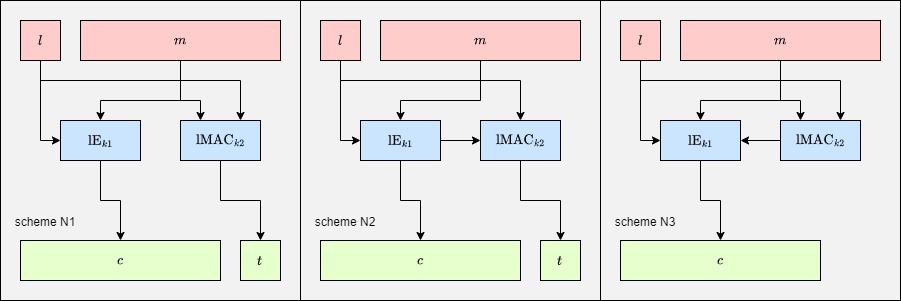
\includegraphics[scale = 0.4]{images/N-schemes.png}
\caption{Adjusted N schemes from \recgc}
\end{figure}

\begin{figure}[H]
    \begin{pchstack}[boxed,center,space=0.5cm]
        \pseudocode[lnstart=-1,linenumbering,head={AE.enc$(\keyinstance,\lockinstance,\messageinstance)$}]{
            (\keyinstance{}1,\keyinstance{}2) \result \keyinstance \\
            \ciphertextinstance' \result \text{E.enc}(\keyinstance{}1,\lockinstance,\messageinstance) \\
            \taginstance \result \text{M.mac}(\keyinstance{}2,\lockinstance,\messageinstance) \\
            \ciphertextinstance \result (\ciphertextinstance',\taginstance)\\
            \pcreturn \ciphertextinstance
        }
        \pseudocode[lnstart=4,linenumbering,head={AE.dec$(\keyinstance,\lockinstance,\ciphertextinstance)$}]{
            (\keyinstance{}1,\keyinstance{}2) \result \keyinstance \\
            (\ciphertextinstance',\taginstance) \result \ciphertextinstance \\
            \messageinstance \result \text{E.dec}(\keyinstance{}1,\lockinstance,\ciphertextinstance') \\
            \taginstance' \result \text{M.mac}(\keyinstance{}2,\lockinstance,\messageinstance) \\
            \pcif \taginstance = \taginstance' : \pcreturn \messageinstance \\
            \pcelse : \pcreturn \invalid
        }
    \end{pchstack}
\caption{Calls based on N1}
\end{figure}

\begin{figure}[H]
    \begin{pchstack}[boxed,center,space=0.5cm]
        \pseudocode[lnstart=-1,linenumbering,head={AE.enc$(\keyinstance,\lockinstance,\messageinstance)$}]{
            (\keyinstance{}1,\keyinstance{}2) \result \keyinstance\\
            \ciphertextinstance' \result \text{E.enc}(\keyinstance{}1,\lockinstance,\messageinstance)\\
            \taginstance \result \text{M.mac}(\keyinstance{}2,\lockinstance,\ciphertextinstance')\\
            \ciphertextinstance \result (\ciphertextinstance',\taginstance)\\
            \pcreturn \ciphertextinstance
        }
        \pseudocode[lnstart=4,linenumbering,head={AE.dec$(\keyinstance,\lockinstance,\ciphertextinstance)$}]{
            (\keyinstance{}1,\keyinstance{}2) \result \keyinstance\\
            (\ciphertextinstance',\taginstance) \result \ciphertextinstance\\
            \messageinstance \result \text{E.dec}(\keyinstance{}1,\lockinstance,\ciphertextinstance')\\
            \taginstance' \result \text{M.mac}(\keyinstance{}2,\lockinstance,\ciphertextinstance')\\
            \pcif \taginstance = \taginstance' : \pcreturn \messageinstance \\
            \pcelse : \pcreturn \invalid
        }
    \end{pchstack}
\caption{Calls based on N2}
\end{figure}

\begin{figure}[H]
    \begin{pchstack}[boxed,center,space=0.5cm]
        \pseudocode[lnstart=-1,linenumbering,head={AE.enc$(\keyinstance,\lockinstance,\messageinstance)$}]{
            (\keyinstance{}1,\keyinstance{}2) \result \keyinstance\\
            \taginstance \result \text{M.mac}(\keyinstance{}2,\lockinstance,\messageinstance)\\
            \messageinstance' \result \messageinstance \concatinate \taginstance\\
            \ciphertextinstance \result E.enc(\keyinstance{}1,\lockinstance,\messageinstance')\\
            \pcreturn \ciphertextinstance
        }
        \pseudocode[lnstart=4,linenumbering,head={AE.dec$(\keyinstance,\lockinstance,\ciphertextinstance)$}]{
            (\keyinstance{}1,\keyinstance{}2) \result \keyinstance\\
            \messageinstance' \result \text{E.dec}(\keyinstance{}1,\lockinstance,\ciphertextinstance)\\
            (\messageinstance,\taginstance) \result \messageinstance'\\
            \taginstance' \result \text{M.mac}(\keyinstance{}2,\lockinstance,\messageinstance)\\
            \pcif \taginstance = \taginstance' : \pcreturn \messageinstance \\
            \pcelse : \pcreturn \invalid
        }
    \end{pchstack}
\caption{Calls based on N3}
\end{figure}

\subsection{Security Bounds}
We define the constructions secure if there is a tight reduction from breaking the loAE-security of the scheme to breaking the loE-security and the loMAC security of the underlying primitives.

\subsection{Comparison with Existing Alternatives}

\section{Use Cases}
should consist of:
\begin{itemize}
	\item possible use cases
\end{itemize}
\subsection{PKE Schemes}

\section{Related Work}
\textbf{Location not final yet}

\section{Conclusion}

\newpage
\printbibliography[heading=bibintoc,title={References}]
\section{Appendix A}
Below is a table which highlights the differences in notation between \pkc{} and \recgc, as well as give the notation I will be using.\\
\begin{tabular}[H]{|c | c | c | c | m{4,5cm}|}
    \hline
    Name   &   \pkc   &   \recgc   &   my notation & rough meaning \\[0.5 ex]
    \hline
    \hline
    message   &   $m$   &   $M$   &   \messageinstance &  message the user sends \\
    \hline
    ciphertext space   &   $\mathcal{C}$   &   -   &   \ciphertextspace & set of all possible ciphertext options \\
    \hline
    ciphertext   &   $c$   &   $C$   &   \ciphertextinstance & encrypted message \\
    \hline
    associated data   &   -   &   $A$   &   \associateddatainstance & data you want to authenticate but not encrypt \\
    \hline
    tag space   &   $\mathcal{C}$   &   -   &   \tagspace & set off all possible tag options \\
    \hline
    tag   &   $c$   &   $T$   &   \taginstance & output of mac function \\
    \hline
    key   &   $k$   &   $K$   &   \keyinstance   & user key \\
    \hline
    nonce space   &   -   &   $\mathcal{N}$   &   \noncespace & set of all nonce options \\
    \hline
    nonce   &   -   &   $n$   &   \nonceinstance & number only used once \\
    \hline
    lock space   &   $\mathcal{T}$   &   -   &   \lockspace & set of all possible lock options \\
    \hline
    lock   &   $t$   &   -   &   \lockinstance & nonce that is bound to the user \\
    \hline
    adversary   &   A   &   $\mathcal{A}$   &   \adversary & the bad guy \\
    \hline
    random sampling   &   $\xleftarrow{\$}$    &   $\twoheadleftarrow$   &   \sample & get a random ellermetn form the set \\
    \hline
    result of randomized function   &   $\xleftarrow{\$}$   &   -   &   \result & get the result of a randomized function with given inputs \\
    \hline
    %Name   &   \pkc   &   \GCrec   &   my notation & rough meaning \\
    %\hline
\end{tabular}

\end{document}

\NeedsTeXFormat{LaTeX2e}
\ProvidesPackage{rutitlepage}[2022/02/21 Mart Lubbers]
\RequirePackage{geometry,graphicx,ifpdf,keyval,iflang}
\def\@rutitleauthors{\@author}
\def\@rutitleauthorstext{Aut\IfLanguageName{dutch}{eu}{ho}r:}
\def\@rutitledate{\@date}
\def\@rutitleinst{Radboud Universit\IfLanguageName{dutch}{eit}{y} Nijmegen}
\def\@rutitletitle{\@title}
\def\@rutitlelayout{twentytwo}
\newif\if@rutitlecolour\@rutitlecolourfalse
\define@key{maketitleru}{authors}{\def\@rutitleauthors{#1}}
\define@key{maketitleru}{authorstext}{\def\@rutitleauthorstext{#1}}
\define@key{maketitleru}{colour}[true]{\@rutitlecolourtrue}
\define@key{maketitleru}{course}{\def\@rutitlecourse{#1}}
\define@key{maketitleru}{date}{\def\@rutitledate{#1}}
\define@key{maketitleru}{institution}{\def\@rutitleinst{#1}}
\define@key{maketitleru}{layout}{\def\@rutitlelayout{#1}}
\define@key{maketitleru}{nextpagenr}{\def\@rutitlenextpagenr{#1}}
\define@key{maketitleru}{others}{\def\@rutitleothers{#1}}
\define@key{maketitleru}{subtitle}{\def\@rutitlesubtitle{#1}}
\define@key{maketitleru}{title}{\def\@rutitletitle{#1}}
\newcommand*{\rutitlepage@printothers}[2]{\textit{#1}\\#2}
\newcommand*{\rutitlepage@sepothers}{\\[\baselineskip]}
\newcommand*{\rutitlepage@others}[2]{%
	\rutitlepage@printothers{#1}{#2}%
	\kernel@ifnextchar,{\rutitlepage@sepothers\rutitlepage@otherslist@}\relax}
\newcommand*{\rutitlepage@otherslist}[1]{%
	\expandafter\rutitlepage@others#1}
\def\rutitlepage@otherslist@,#1{\rutitlepage@otherslist{{#1}}}
\newcommand{\rutitle@layout@twentytwo}[0]{
	\newgeometry{left=25mm,top=25mm,right=15mm,bottom=10mm,hmarginratio=1:1}
	\begin{titlepage}%
		\null\vfill%
		\parindent0pt
		\ifdefined\@rutitlecourse\textsc{\LARGE\@rutitlecourse}\\[1.5cm]\fi
		{\Huge\bfseries\@rutitletitle}%
		\ifdefined\@rutitlesubtitle{\\[2\baselineskip]\large\itshape\@rutitlesubtitle\/}\fi\\[4\baselineskip]
		{\Large\scshape\@rutitleauthors}\\[\baselineskip]
		{\large\@rutitledate}
		\vfill

		\ifdefined\@rutitleothers\rutitlepage@otherslist\@rutitleothers\fi
		\vfill

		\hfill
		\ifpdf\includegraphics[width=80mm]{rutitlepage-logo-\IfLanguageName{dutch}{nl-}{}\if@rutitlecolour cmyk\else bw\fi.pdf}\\
		\else\includegraphics[width=80mm]{rutitlepage-logo-\IfLanguageName{dutch}{nl-}{}\if@rutitlecolour cmyk\else bw\fi.eps}\\
		\fi
	\end{titlepage}
	\restoregeometry%
}
\newcommand{\rutitle@layout@seventeen}[0]{
	\newgeometry{left=25mm,top=25mm,right=15mm,bottom=10mm,hmarginratio=1:1}
	\begin{titlepage}%
		\null\vfill%
		\parindent0pt
		{\Huge\bfseries\@rutitletitle}%
		\ifdefined\@rutitlesubtitle{\\[2\baselineskip]\large\itshape\@rutitlesubtitle\/}\fi\\[4\baselineskip]
		{\Large\scshape\@rutitleauthors}\\[\baselineskip]
		{\large\@rutitledate}
		\vfill

		\ifdefined\@rutitleothers\rutitlepage@otherslist\@rutitleothers\fi
		\vfill

		\hfill
		\ifpdf\includegraphics[width=80mm]{rutitlepage-logo-\IfLanguageName{dutch}{nl-}{}\if@rutitlecolour cmyk\else bw\fi.pdf}\\
		\else\includegraphics[width=80mm]{rutitlepage-logo-\IfLanguageName{dutch}{nl-}{}\if@rutitlecolour cmyk\else bw\fi.eps}\\
		\fi
	\end{titlepage}
	\restoregeometry%
}
\newcommand{\rutitle@layout@traditional}[0]{
	\newgeometry{hmarginratio=1:1}
	\begin{titlepage}
		\begin{center}
			\ifdefined\@rutitlecourse\textsc{\LARGE\@rutitlecourse}\\[1.5cm]\fi
			\ifpdf\includegraphics[height=150pt]{rutitlepage-logo.pdf}\\
			\else\includegraphics[height=150pt]{rutitlepage-logo.eps}\\
			\fi
			\vspace{0.4cm}
			\textsc{\Large\@rutitleinst}\\[1cm]
			\hrule
			\vspace{0.4cm}
			\textbf{\large\@rutitletitle}\\[0.4cm]
			\hrule
			\ifdefined\@rutitlesubtitle
				\vspace{0.4cm}
				\textit{\@rutitlesubtitle}\\[1cm]
			\else
				\vspace{2cm}
			\fi
			\begin{minipage}[t]{0.45\textwidth}
				\begin{flushleft}\large
					\textit{\@rutitleauthorstext}\\
					\@rutitleauthors{}
				\end{flushleft}
			\end{minipage}
			\begin{minipage}[t]{0.45\textwidth}
				\begin{flushright}\large
					\ifdefined\@rutitleothers
					\renewcommand{\rutitlepage@printothers}[2]{\textit{##1}\\##2}
					\renewcommand{\rutitlepage@sepothers}[0]{

						\vspace{8mm}}
					\rutitlepage@otherslist\@rutitleothers
					\fi
				\end{flushright}
			\end{minipage}
			\vfill
			{\large\@rutitledate}
		\end{center}
	\end{titlepage}
	\restoregeometry%
}
\newcommand{\maketitleru}[1][]{
	\setkeys{maketitleru}{#1}
	\ifcsname%
		rutitle@layout@\@rutitlelayout\endcsname
		\expandafter\csname rutitle@layout@\@rutitlelayout\endcsname
	\else
		\PackageError{rutitlepage}
			{Unknown layout `\@rutitlelayout'.}
			{The `layout' key of \maketitleru\space contained an unknown layout.\MessageBreak{}
			 Check the package documentation for the possible layouts.}
	\fi
	\ifdefined\@rutitlenextpagenr\setcounter{page}{\@rutitlenextpagenr}\fi%
}